\section{Durchführung}
\label{sec:Durchführung}
\subsection{Bestimmung der Zeitkonstante anhand der Aufladekurve}
Zunächst wird die Zeitkonstante eines RC-Gliedes mithilfe des in Abbildung \ref{fig:aufbau_a} beschriebenen Aufbaus ermittelt.
\begin{figure}[H]
  \centering
  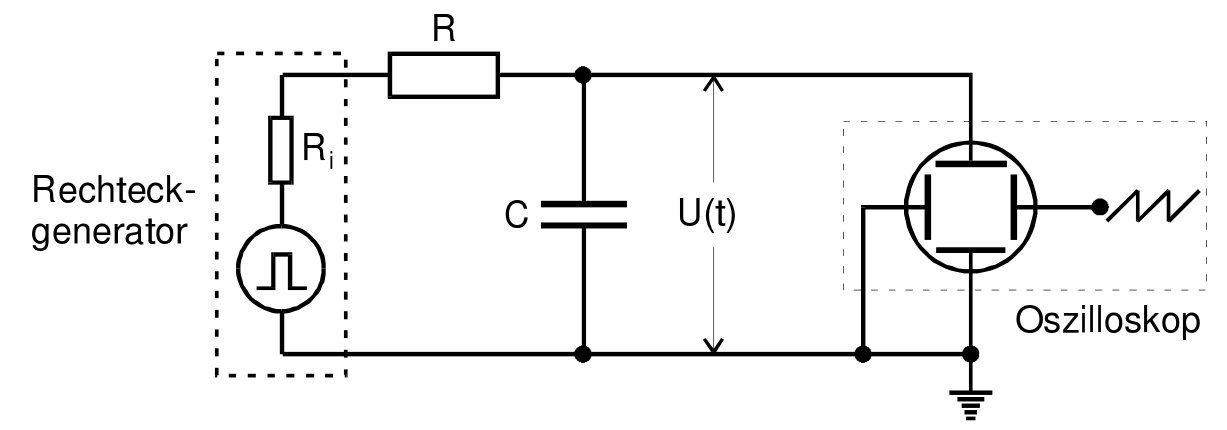
\includegraphics[height=5cm]{aufbau_a.png}
  \caption{Schaltung zur Bestimmung der Zeitkonstante eines RC-Gliedes. \cite{sample}}
  \label{fig:aufbau_a}
\end{figure}
Hierbei wird an einem in Reihe geschalteten Widerstand mit Kondensator eine Rechteckspannung der Frequenz $\omega$ angelegt.
Die am Kondensator entstehende Spannung $U_c$ wird mit einem digitalen Oszilloskop gemessen.
Um das Oszilloskop auf die Nullspannung des Kondensators zu eichen, wird die Rechteckspannung zunächst auf eine zu $\frac{1}{RC}$ kleine Frequenz eingestellt, so dass sich der Kondensator nahezu vollständig entladen kann.
Der Y-Achsenabschnitt wird dementsprechend auf die Nullspannung eingestellt.\\
Im Folgenden wird die Frequenz der Rechteckspannung so eingestellt, so dass eine aussagekräftige Aufladekurve des Kondensators abgelesen werden kann.
Hierbei soll einerseits eine Änderung der Spannung von einem Faktor von mindestens 5 erkennen zu sein, andererseits wird darauf geachtet, dass die Spannung nicht zu lange im niedrigen Bereich ist, da dieser Bereich vom Oszilloskop nicht genau genug angezeigt werden kann.
Die Entladekurve wird schlussendlich digital abgespeichert, so dass $(t, U(t))$ Wertepaare abgelesen werden können.

\subsection{Messung der Spannungsamplitude und Phasenverschiebung in Abhängigkeit von der Frequenz}
Im zweiten Abschnitt der Versuchs wird die Spannungsamplitude der Kondensatorspannung sowie dessen Phasenverschiebung zur angelegten Sinusspannung untersucht.
Beide sind, wie in der Theorie geschrieben, von der angelegten Frequenz $\omega$ abhängig.
Hierzu wird eine Schaltung wie in Abbildung \ref{fig:aufbau_b} aufgebaut.
\begin{figure}[H]
  \centering
  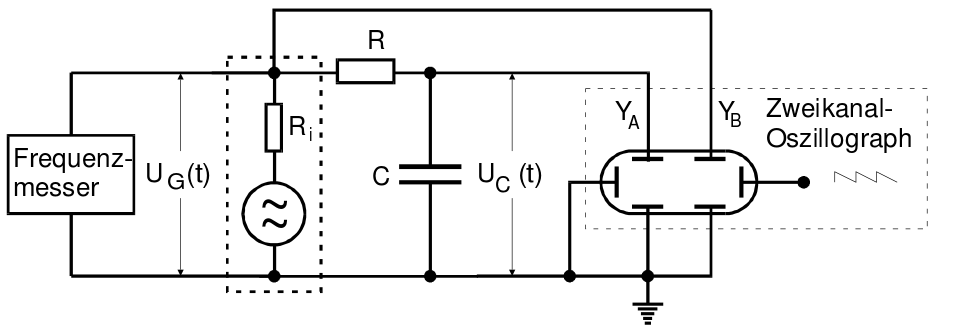
\includegraphics[height=5cm]{aufbau_b.png}
  \caption{Schaltung zur Messung der Spannungsamplitude und Phasenverschiebung in Abhängigkeit von der Frequenz. \cite{sample}}
  \label{fig:aufbau_b}
\end{figure}
Der Widerstand und der Kondensator werden erneut parallel geschaltet, die angelegte Spannung ist dieses mal eine Sinusspannung.
Mithilfe eines Zweikanal-Oszillographens werden sowohl die am Kondensator anliegende Spannung $U_c$ sowie die angelegte Sinusspannung $U_G$ gemessen und angezeigt.
Beide Kurven werden widerum so geeicht, dass der Y-Achsenabschnitt bei 0 der Nullspannung entspricht.
Unter Zuhilfenahme der Cursor-Funktion werden für verschiedene am Frequenzgenerator eingestellte Frequenzen die Phasendifferenzen zwischen $U_c$ und $U_G$ bestimmt, indem der Abstand zwischen zwei Nulldurchläufgen gleicher Phase abgelesen wird.
Gleichzeitig wird mit der Cursor-Funktion der Spannungsabstand der Kondensatorspannung von Peak zu Peak abgelesen und notiert.
Die betrachteten Frequenzen werden so gewählt, so dass diese in einem Bereich von vier Zehnerpotenzen liegen.
Bei auffälligen Werteänderungen werden genauere Messungen für kleinere Frequenzabstände durchgeführt.
\subsection{Nutzung des RC-Gliedes zur Integration}
Zum Schluss des Versuchs wird die in der Theorie beschriebene Fähigkeit des RC-Gliedes zur Integration untersucht.
Dazu wird die in Abbildung \ref{fig:aufbau_b} Schaltung genutzt.
Die Frequenz $\omega$ wird hinreichend groß gewählt, so dass sowohl die Bedingung $ \omega \gg \frac{1}{RC}$ erfüllt, aber auch die Stromamplitude $U_c$ weiterhin gut messbar ist.
Die Integrationseigenschaft wird nun anhand einer angelegten Rechteckspannung, einer Sinusspannung sowie einer Dreieckspannung überprüft.
